\documentclass[UTF8,a4paper,12pt]{ctexart}
\usepackage{amsmath}
\numberwithin{equation}{section}
\allowdisplaybreaks[4]       %多行公式中换页
\usepackage{array}
\usepackage{caption}
\usepackage{amssymb}
\usepackage{tikz}
\usepackage{amsthm}
\usepackage{mathrsfs}
\usepackage{dutchcal}
\usepackage{color}
\usepackage{graphicx}    %插入图片
\usepackage{times}
\usepackage{mathptmx}
\usepackage{fancyhdr} %页眉页脚
\usepackage{booktabs}  %三线表
\usepackage[T1]{fontenc}
\usepackage{enumerate}
\usepackage{physics}
\usepackage{siunitx}
\usepackage[ruled,vlined]{algorithm2e}
\usepackage{subcaption}
\usepackage{bicaption}
\usepackage{appendix}


% 中文字体设置,不设置时默认为linux系统自带的宋体fandol-song
%\usepackage{xeCJK}
%\setCJKmainfont{Noto Serif CJK SC} % 如果有生僻字,可以换用思源宋体为主要字体
%\setCJKsansfont{Noto Sans CJK SC}
%\setCJKmonofont{Noto Sans Mono CJK SC}

% 英文字体设置
%\setmainfont{Times New Roman}  % 默认字体也是Roman字体,可以根据自己喜好设置
%\setsansfont{Arial}            % 默认的无衬线字体跟Arial非常接近,可以根据自己喜好设置


% 参考文献设置
\usepackage[backend=biber,style=gb7714-2015,maxnames=3]{biblatex}
\renewcommand{\bibfont}{\small} % 文献表字号
\setlength{\bibitemsep}{0pt}    % 文献表条目间的间距
\addbibresource{main.bib}       % 导入参考文献数据库


% 页面版心大小
\setlength{\textheight}{22cm}
\setlength{\textwidth}{15cm}

% 页边距设置
\setlength{\voffset}{-1.14cm}
\setlength{\hoffset}{-0.57cm}
%\setlength{\headheight}{14.48167pt} 
\setlength{\headheight}{1cm}
\setlength{\topmargin}{0cm}
%\setlength{\headsep}{2.9cm}
\setlength{\headsep}{1.8cm}
\setlength{\footskip}{1.2cm}


% 页眉页脚设置
\pagestyle{fancy}
\fancyhf{}
\fancyfoot[C]{\thepage}
% 只需要区分fancy和empty页面,每章的页眉页脚需手动定义
\fancypagestyle{plain}{
  \pagestyle{fancy}     % 将plain页面格式替换为fancy,确保目录页有页眉
}
\fancyhfinit{\small} % 页眉页脚字号

% 双线页眉
\makeatletter
\def\headrule{{\if@fancyplain\let\headrulewidth\plainheadrulewidth\fi%
\hrule\@height 1.5pt \@width\headwidth\vskip1.5pt%上面线为1pt粗
\hrule\@height 0.5pt\@width\headwidth  %下面0.5pt粗
\vskip-2\headrulewidth\vskip-1pt}      %两条线的距离1pt
  \vspace{6mm}}     %双线与下面正文之间的垂直间距
\makeatother


% 行距
\usepackage{setspace}
\setlength{\baselineskip}{20pt}
\newcommand*{\circled}[1]{\lower.7ex\hbox{\tikz\draw (0pt, 0pt)%
    circle (.5em) node {\makebox[1em][c]{\small #1}};}}


% 目录设置
\usepackage{hyperref}  
\hypersetup{hidelinks}

\usepackage{tocloft} 
\renewcommand{\cftsecleader}{\cftdotfill{\cftdotsep}} %为目录中section补上引导点
\usepackage{titletoc}
\titlecontents{section}[0pt]
              {\addvspace{6pt}\filright\large\bf} %要将ABSTRACT的字体也替换为Arial的话,在本括号中末尾加上\ttfamily\songti
              {\contentspush{\thecontentslabel \quad }} %
              {}{\titlerule*[8pt]{.}\contentspage}
\setlength{\cftbeforesubsecskip}{6pt}
\setlength{\cftbeforesubsubsecskip}{6pt}

% 目录缩进
\setlength{\cftsubsecindent}{1em}
\setlength{\cftsubsubsecindent}{2em}

% 目录字体
\renewcommand{\cftsubsecfont}{\normalsize}
\renewcommand{\cftsubsubsecfont}{\small}


% 图表编号
\captionsetup[figure][bi-second]{name=Figure} %设置图的英文编号前缀
\captionsetup[table][bi-second]{name=Table} %设置表的英文编号前缀
\numberwithin{equation}{section}%公式按章节编号
\numberwithin{figure}{section}%图表按章节编号
\numberwithin{table}{section}
\renewcommand {\thefigure} {\thesection{}-\arabic{figure}}%设定图片的编号。这样设置的实现效果为图1-1
\renewcommand {\thetable} {\thesection{}-\arabic{table}}


% 图/表标题格式
\captionsetup{font={small,bf},labelsep=quad,justification=centering} 
\captionsetup[subfigure]{labelfont=normalfont,textfont=normalfont} % 子图题不加粗


% 浮动体间距
%\setlength{\intextsep}{6pt}    % h浮动体与上下文间距
%\setlength{\floatsep}{6pt}     % 浮动体之间的间距
%\setlength{\textfloatsep}{6pt} % t/b浮动体与正文邻接间距


% 表内字体
\usepackage[captionskip=6pt]{floatrow}
\floatsetup[table]{font={small},capposition=top}


% 各级标题格式
\ctexset{section={
  format={\heiti \zihao{3} \bfseries \center},
  number={第\chinese{section}章}
}}
\usepackage{titlesec}
\titlespacing*{\section}{0pt}{24pt}{18pt}
\titlespacing{\subsection}{0pt}{24pt}{12pt}
\titlespacing{\subsubsection}{0pt}{12pt}{6pt}
\titleformat*{\subsection}{\heiti\large\bfseries}
\titleformat*{\subsubsection}{\heiti\normalsize\bfseries}


% autoref中文名称
\def\equationautorefname{式}
\def\footnoteautorefname{脚注}
\def\itemautorefname{项}
\def\figureautorefname{图}
\def\tableautorefname{表}
%\def\partautorefname{篇}
\def\appendixautorefname{附录}
%\def\chapterautorefname{章} % 不使用chapter,而使用section作为章
\def\sectionautorefname{} % 由于已经修改章节名称为第X章,应该在autoref中不加前缀
\def\subsectionautorefname{节}
\def\subsubsectionautorefname{小节}
\renewcommand{\algorithmcfname}{算法}
\renewcommand{\algorithmautorefname}{算法}


% 盲审模式控制
\newif \ifreview
%\reviewtrue     %开启盲审模式,反之注释掉
\reviewfalse    %关闭盲审模式


% 打印模式控制(需要在章节划分处使用\clearsection命令)
\newif \ifprint
%\printtrue      %打印模式
\printfalse     %非打印模式,建议用于生成电子版

\ifprint
\newcommand{\clearsection}{\clearpage \ifodd\value{page}\else \thispagestyle{empty}\hbox{}\newpage\fi} % 打印模式下,每章右页起
\else
\newcommand{\clearsection}{\clearpage} % 非打印模式,连续排版
\fi




\begin{document}

\thispagestyle{empty}

\renewcommand{\headrulewidth}{0pt}
\begin{figure}[htb] 
\center{
\includegraphics[width=3.5cm]  {fig/fig1.png}} 
\end{figure}

\begin{center}
\songti \zihao{-2} 上海交通大学学位论文
\end{center}
%该页为中文扉页。无需页眉页脚,纸质论文应装订在右侧
~\\
\begin{center}
\songti \zihao{1} \textbf{上海交通大学学位论文模板}
\end{center}
%中文论文标题,1行或2行,宋体,加粗,二号,居中。论文题目不得超过36个汉字
~\\
~\\
~\\
\begin{center}
\setstretch{1.725}
\heiti \zihao{4}
\begin{tabular}{l}
\ifreview
\textbf{姓\quad  名:}\\    %不要填写
\textbf{学\quad  号:}\\    %不要填写
\textbf{导\quad  师:}\\    %不要填写
\else
\textbf{姓\quad  名:}\\
\textbf{学\quad  号:}\\
\textbf{导\quad  师:}\\
\fi
\textbf{学\quad  院: }\\
\textbf{学科/专业名称:}\\
\textbf{申请学位层次:}\\
\end{tabular}
\end{center}
~\\
~\\
\begin{center}
\songti \zihao{4} \textbf{20XX年XX月}
\end{center}

\clearsection




\thispagestyle{empty}
\begin{center}
\setstretch{1.725}
\zihao{4}
\textbf{
A Dissertation Submitted to \\
Shanghai Jiao Tong University for Bachelor Degree}
\end{center}
~\\
\begin{center}
\zihao{-2}\textbf{
DISSERTATION TEMPLATE FOR BACHELOR DEGREE OF ENGINEERING IN \\
SHANGHAI JIAO TONG UNIVERSITY}
\end{center}
%英文论文标题:大写,Times New Roman,加粗,14 points,居中
~\\
~\\
~\\
\begin{center}
\setstretch{1.725}
\zihao{3} 
\ifreview
\textbf{Author:}  \\   %不要填写
\textbf{Supervisor:}    %不要填写
\else
\textbf{Author:}  XXXXXXX\\
\textbf{Supervisor:}   XXXXXXX
\fi
\end{center}
~\\
~\\
~\\
~\\
\begin{center}
\setstretch{1.725}
\zihao{3} 
School of XXXXXXX \\
Shanghai Jiao Tong University \\
Shanghai, P.R.China \\
June 28$^{\mathrm{th}}$, 2021  
\end{center}

\clearsection

\ifreview
\else
\thispagestyle{empty}
\begin{center}
\heiti \zihao{3}\textbf{
上海交通大学\\
学位论文原创性声明}
\end{center}

\zihao{-4}
本人郑重声明:所呈交的学位论文,是本人在导师的指导下,独立进行研究工作所取得的成果。除文中已经注明引用的内容外,本论文不包含任何其他个人或集体已经发表或撰写过的作品成果。对本文的研究做出重要贡献的个人和集体,均已在文中以明确方式标明。本人完全知晓本声明的法律后果由本人承担。

\begin{flushright}
\begin{tabular}{l}
\zihao{4}
学位论文作者签名:
\begin{minipage}{30mm}
\quad % 电子签名图片
\end{minipage}\\
\zihao{4}
日期:\qquad 年\quad 月\quad 日
\end{tabular}
\end{flushright}

~\\
\begin{center}
\heiti \zihao{3}\textbf{
上海交通大学\\
学位论文使用授权书}
\end{center}

本人同意学校保留并向国家有关部门或机构送交论文的复印件和电子版,允许论文被查阅和借阅。\\
本学位论文属于 :\par
$\square$\textbf{公开论文}\par
%\vspace{-\baselineskip}\textbf{\checkmark}\par %在上一行的方框内打勾
$\square$\textbf{内部论文},保密$\square$1年/$\square$2年/$\square$3年,过保密期后适用本授权书。\par
$\square$\textbf{秘密论文},保密\_\_\_年(不超过10年),过保密期后适用本授权书。\par
$\square$\textbf{机密论文},保密\_\_\_年(不超过20年),过保密期后适用本授权书。\par
(请在以上方框内选择打“\textbf{\checkmark}”)\\

\begin{flushright}
\zihao{4}
\begin{tabular}{l l}
学位论文作者签名:
\begin{minipage}{35mm}
\quad % 电子签名图片
\end{minipage}
&指导教师签名:
\begin{minipage}{22mm}
\quad % 电子签名图片
\end{minipage} \\
日期:\qquad 年\quad 月\quad 日 &日期:\qquad 年\quad 月\quad 日\\
\end{tabular}
\end{flushright}

\clearsection
\fi

\pagenumbering{Roman}
\fancyhead[LH]{上海交通大学学位论文}
\fancyhead[RH]{}

\addcontentsline{toc}{section}{摘\quad 要}
\section*{摘\quad 要}
%摘要:二字间空一格,黑体16磅加粗居中,单倍行距,段前24磅,段后18磅。

\hspace{8mm}学位论文是本科生从事科研工作的成果的主要表现,集中表明了作者在研究工作中获得的新的发明、理论或见解,也是科研领域中的重要文献资料和社会的宝贵财富。\par 
为了提高本科生学位论文的质量,做到学位论文在内容和格式上的规范化与统一化,特制作本模板。\\
~\\
\textbf{关键词}:学位论文,论文格式,规范化,模板\\
%关键字:宋体12磅,行距20磅,段前段后0磅,关键字之间用逗号隔开,关键词三个字加粗。

\clearsection




\addcontentsline{toc}{section}{ABSTRACT}
\section*{\textsf{ABSTRACT}}
%ABSTRCT:Arial 16磅加粗居中,单倍行距,段前24磅,段后18磅

\hspace{8mm}As a primary means of demonstrating research findings for undergraduate students, dissertation is a systematic and standardized record of the new inventions, theories or insights obtained by the author in the research work. It can not only function as an important reference when students pursue further studies, but also contribute to scientific research and social development.\par 
This template is therefore made to improve the quality of undergraduates’ dissertation and to further standardize it both in content and in format.\\
%英文摘要内容:Times New Roman 12磅,行距20磅段前段后0磅
~\\ 
\textbf{Key words}: dissertation, dissertation format, standardization, template
%Keywords:Times New Roman 12磅,行距20磅, “key words” 两词加粗

\clearsection

\renewcommand\contentsname{\heiti \textbf{目\quad 录}}

\begin{center}
\tableofcontents
\end{center}

\clearsection

\pagenumbering{arabic}


\fancyhead[LH]{上海交通大学学位论文}
\fancyhead[RH]{第一章\quad 绪论}

\section{绪论}
\subsection{引言}
学位论文……
\subsection{本文主要研究内容}
本文……
\subsection{本文研究意义}
本文……
\subsection{本章小结}
本文……

\clearsection

\fancyhead[LH]{上海交通大学学位论文}
\fancyhead[RH]{第二章\quad 正文文字格式}
\section{正文文字格式}
\subsection{论文正文}
论文正文是主体,一般由标题、文字叙述、图、表格和公式等部分构成。一般可包括理论分析、计算方法、实验装置和测试方法,经过整理加工的实验结果分析和讨论,与理论计算结果的比较以及本研究方法与已有研究方法的比较等,因学科性质不同可有所变化。\par
论文内容一般应由十个主要部分组成,依次为:⒈封面,⒉中文摘要,⒊英文摘要,⒋目录,⒌符号说明,⒍论文正文,⒎参考文献,⒏附录,⒐致谢,⒑攻读学位期间发表的学术论文目录。\par
以上各部分独立为一部分,每部分应从新的一页开始,且纸质论文应装订在论文的右侧。\par
\subsection{字数要求}
\subsubsection{本科论文字数要求}
各学科和学院自定。理工科研究类论文一般不少于2万字,设计类一般不少于1.5万字;医科、文科类论文一般不少于1万字。
\subsection{引用格式}
引用\cite{label1}
\citet{label2}提出 \dots
\citet{label3}提出 \dots

\subsection{本章小结}
本章介绍了……

\clearsection

\fancyhead[LH]{上海交通大学学位论文}
\fancyhead[RH]{第三章\quad 图表、公式格式}
\section{图表、公式格式}
\subsection{图表格式}

\begin{figure}[htb] 
\center{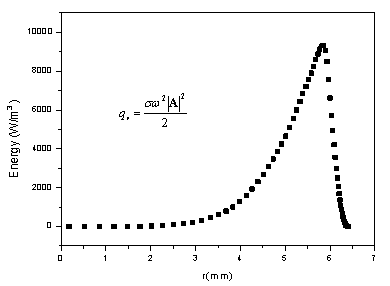
\includegraphics[width=0.95\textwidth]  {fig/fig2.png}} 
\bicaption{内热源沿径向的分布}{Distribution of internal heat sources along the radial direction}
\end{figure}



\begin{table}[!htbp]
    \centering
    \bicaption{高频感应加热的基本参数}{Basic parameters of high frequency induction heating}
    \begin{tabular}{cccc}
    \toprule
    感应频率 &感应发生器功率 & 工件移动速度  &感应圈与零件间隙\\
    (KHz)&($\% \times$80Kw) &(mm/min)  &(mm)\\
    \midrule
    250 &88 &5900 &1.65\\
    250 &88 &5900 &1.65\\
    250 &88 &5900 &1.65\\
    250 &88 &5900 &1.65\\
    \bottomrule
    \end{tabular}
\end{table}


\begin{table}
    \centering
    \begin{tabular}{cccc}
    \multicolumn{4}{l}{\textbf{续表}}
    \vspace{6pt}\\
    \toprule
    感应频率 &感应发生器功率 & 工件移动速度  &感应圈与零件间隙\\
    (KHz)&($\% \times$80Kw) &(mm/min)  &(mm)\\
    \midrule
    250 &88 &5900 &1.65\\
    250 &88 &5900 &1.65\\
    \bottomrule
    \end{tabular}
\end{table}
%表格太大需要转页时,需要在续表上方注明“续表”,表头也应重复排出。


\subsection{公式格式}
\vspace{-10mm}
\begin{eqnarray}
\frac{1}{\mu} \nabla^2A - j \omega \sigma A -\nabla(\frac{1}{\mu}) \times(\nabla \times A)+J_0=0
\end{eqnarray}

\subsection{本章小结}
\begin{figure}[htb] 
    \center{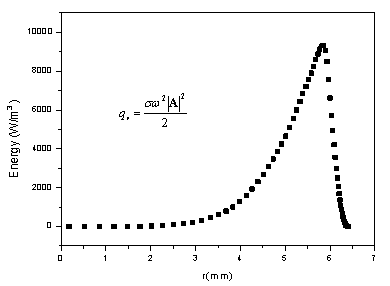
\includegraphics[width=0.95\textwidth]  {fig/fig2.png}} 
    \bicaption{内热源沿径向的分布}{Distribution of internal heat sources along the radial direction}
\end{figure}
本章介绍了……

\clearsection

\fancyhead[LH]{上海交通大学学位论文}
\fancyhead[RH]{第四章\quad 全文总结}
\section{全文总结}

\subsection{主要结论}
本文主要……
\begin{figure}[htb] 
    \center{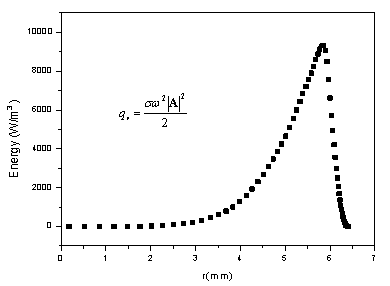
\includegraphics[width=0.95\textwidth]  {fig/fig2.png}} 
    \bicaption{内热源沿径向的分布}{Distribution of internal heat sources along the radial direction}
    \end{figure}
\subsection{研究展望}

更深入的研究……

\clearsection


\fancyhead[LH]{上海交通大学学位论文}
\fancyhead[RH]{参考文献}


%\nocite{*}     % 添加未引到的参考文献


% 常见问题:引用网络文献时缺少引用日期。
% 解决方案:使用@online而非@misc,并且添加urldate={20xx-xx-xx}字段

\begin{center}
\setstretch{1.15}
\printbibliography[heading=bibintoc, title={参\quad 考\quad 文\quad 献}]
\end{center}

\clearsection

\fancyhead[LH]{上海交通大学学位论文}
\fancyhead[RH]{附录1}

\addcontentsline{toc}{section}{符号与标记(附录1)}
\section*{符号与标记(附录1)}

\clearsection

\ifreview
\fancyhead[LH]{上海交通大学学位论文}
\fancyhead[RH]{学术论文和科研成果目录}

\addcontentsline{toc}{section}{攻读学位期间学术论文和科研成果目录}
\section*{攻读学位期间学术论文和科研成果目录}

%盲审版本
发表学术论文及参与科研情况等仅以第几作者注明即可,不要出现作者或他人姓名

\clearsection
\else
\fancyhead[LH]{上海交通大学学位论文}
\fancyhead[RH]{学术论文和科研成果目录}

\addcontentsline{toc}{section}{攻读学位期间学术论文和科研成果目录}
\section*{攻读学位期间学术论文和科研成果目录}

[1] 张三,李四. …… (已录用)

\clearsection
\fi

\ifreview
\else

\fancyhead[LH]{上海交通大学学位论文}
\fancyhead[RH]{致谢}

\addcontentsline{toc}{section}{致\qquad 谢}
\section*{致\qquad 谢}
~\par   % 这里空一行
致谢主要感谢导师和对论文工作有直接贡献和帮助的人士和单位。致谢言语应谦虚诚恳,实事求是。

\clearsection
\fi

\pagenumbering{arabic}
\fancyhead[LH]{上海交通大学学位论文}
\fancyhead[RH]{}
\section*{NUMERICAL SIMULATION OF HOMOGENEOUS CHARGE COMPRESSION IGNITION COMBUSTION FUELED WITH DIMETHYL ETHER}%英文大摘要标题

\hspace{8mm}HCCI (Homogenous Charge Compression Ignition) combustion has advantages in terms of efficiency and reduced emission. HCCI combustion can not only ensure both the high economic and dynamic quality of the engine, but also efficiently reduce the NOx and smoke emission. Moreover, one of the remarkable characteristics of HCCI combustion is that the ignition and combustion process are controlled by the chemical kinetics, so the HCCI ignition time can vary significantly with the changes of engine configuration parameters and operating conditions. ……%(英文大摘要正文)

\clearsection


\end{document} 